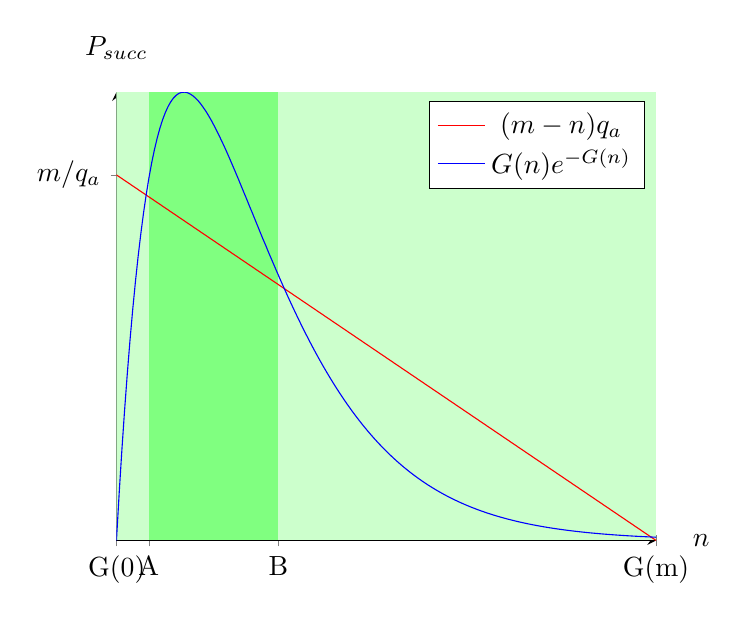
\begin{tikzpicture}
\begin{axis}[axis lines=middle,samples=200
        ,ylabel=$P_{succ}$
        ,xlabel=$n$
        ,every axis x label/.style={
          at={(ticklabel* cs:1.05)},
            anchor=west,
          },
        every axis y label/.style={
          at={(ticklabel* cs:1.05)},
            anchor=south,
          },
        ,xtick=data,
        ,xtick={0.001,0.12,0.6,2}
        ,xticklabels={G(0),A, B,G(m)}
        ,ytick=data,
        ,ytick={0.3}
        ,yticklabels={$m/q_a$}
        ]
			\fill[green!20]
				(axis cs:0,0) --
				(axis cs:0.12,0) --
				(axis cs:0.12,2) --
				(axis cs:0,2) --
				cycle;
			\fill[green!50]
				(axis cs:0.12,0) --
				(axis cs:0.6,0) --
				(axis cs:0.6,2) --
				(axis cs:0.12,2) --
				cycle;
			\fill[green!20]
				(axis cs:0.6,0) --
				(axis cs:2,0) --
				(axis cs:2,2) --
				(axis cs:0.6,2) --
				cycle;
      \addplot[red,domain=0:2] {0.15*(2-x)};
      \addplot[blue,domain=0:2] {4*x*e^(-4*x)};
			\addlegendentry{$(m-n)q_a$}
			\addlegendentry{$G(n)e^{-G(n)}$}
    \end{axis}\end{tikzpicture}
